\documentclass[tikz]{standalone}

%!TEX root = main.tex

% mytikzset
\usepackage{tikz}
\usetikzlibrary{positioning,arrows,shapes,patterns}
\usetikzlibrary{decorations.pathmorphing}
\usetikzlibrary{decorations.markings}
\usetikzlibrary{decorations.pathreplacing}
\usetikzlibrary{calc}
\usetikzlibrary{patterns}
\usetikzlibrary{decorations.markings}
\usetikzlibrary{petri}

\tikzset{
  vector/.style={thick,double,draw=black, postaction={decorate},
    decoration={markings,mark=at position .6 with {\arrow[black,scale=0.4]{triangle 45}}}},
  axial/.style={thick,double,densely dashed,draw=black, postaction={decorate},
    decoration={markings,mark=at position .6 with {\arrow[black,scale=0.4]{triangle 45}}}},
  gluon/.style={decorate, draw=black,
    decoration={coil,aspect=0.3,segment length=5pt,amplitude=3pt}},
  pseudo/.style={thick, dashed, draw=black, postaction={decorate},
    decoration={markings,mark=at position .6 with {\arrow[red,scale=0.5]{triangle 45}}}},
  scalar/.style={thick,draw=black, postaction={decorate},
    decoration={markings,mark=at position .6 with {\arrow[black,scale=0.5]{triangle 45}}}},
  cut/.style={draw=black, decorate, decoration={snake, segment length=1mm, amplitude=0.2mm}}
}


\usepackage{amsfonts}
\newcommand{\Po}{\ensuremath{\mathbb{P}}}

\begin{document}
\nopagecolor
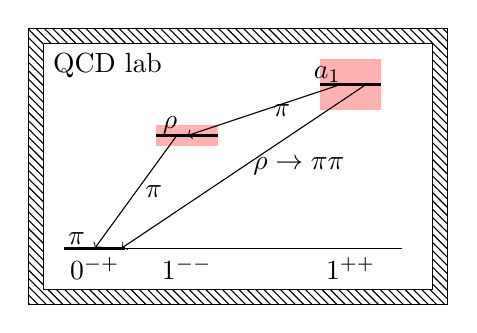
\begin{tikzpicture}[x=1.3cm, y = 1.3cm]
  \newcommand\dxh{0.3}
  \newcommand\eps{0.01}
  \newcommand\drawlevel[1]{
    \draw[very thick] (#1) -- ++(\dxh,0);
    \draw[very thick] (#1) -- ++({-\dxh},0);
  }
  \newcommand\drawbox[3]{
    \fill[red, fill opacity=0.3] (#1)++(#2,#3) rectangle ++(-2*#2,-2*#3);
  }

  \draw[pattern=north west lines] (-0.5-0.3/2,2.0+0.3/2) -- ++(3.8+0.3,0) -- ++(0,-2.4-0.3) -- ++(-3.8-0.3,0) -- ++(0,2.4+0.3);
  \draw[fill=white,very thin] (-0.5,2.0) -- ++(3.8,0) -- ++(0,-2.4) -- ++(-3.8,0) -- ++(0,2.4) node[below right] {QCD lab};


  \node[coordinate] (v0) at (0,0) {};
  \node[coordinate] (v1) at (0.9,1.1) {};
  \node[coordinate] (v2) at (2.5,1.6) {};

  \draw[very thin] (v0) -- (3.0,0);

  \drawbox{v1}{\dxh}{0.1}
  \drawbox{v2}{\dxh}{0.25}
  %
  \drawlevel{v0}
  \drawlevel{v1}
  \drawlevel{v2}
%
  \node[left, yshift=1.3mm] at (v0) {$\pi$};
  \node[left, yshift=1.3mm] at (v1) {$\rho$};
  \node[left, yshift=1.3mm] at (v2) {$a_1$};
%
\node[] at (0.0,-0.2) {$0^{-+}$};
\node[] at (0.9,-0.2) {$1^{--}$};
\node[] at (2.5,-0.2) {$1^{++}$};
  %
  \draw[->] (v2)++(-0.1,0) -- node[right] {$\pi$} (v1);
  \draw[->] (v1)++(-0.1,0) -- node[right] {$\pi$} (v0);
  \draw[->] (v2)++(\dxh/2,0) -- node[right] {$\rho\to\pi\pi$} (0.26,0);
\end{tikzpicture}
\end{document}
